\documentclass[12pt]{article}

\usepackage{amssymb, latexsym, amsmath}
\usepackage[utf8]{inputenc}
\usepackage{graphicx, float, subcaption}
\usepackage{color}
\usepackage{geometry}
\usepackage{hyperref}
\usepackage{slashed}
\usepackage{mathrsfs}
\usepackage{dsfont}


\usepackage{tikz}
\usetikzlibrary{shapes,arrows,positioning,automata,backgrounds,calc,er,patterns}

\bibliographystyle{unsrt}

\title{\textbf{Report: Finding the Higgs Boson with Deep Learning}\\
ASTR598: Topics in Theoretical Astrophysics\\
Winter 2019}
\author{Stephan Hagel\\Student Number: 1870562\\sthagel@uw.edu}
\date{}

\renewcommand{\phi}{\varphi}
\renewcommand{\epsilon}{\varepsilon}
\renewcommand{\mathbb}{\mathds}

\newcommand{\unity}{\mathds{1}}
\newcommand{\tr}{\operatorname{tr}}
\newcommand{\dd}{\mathrm{d}}
\newcommand{\levi}{\varepsilon_{ijk}}
\newcommand{\leviup}{\varepsilon^{ijk}}
\newcommand{\vectz}[2]{\begin{pmatrix}	#1\\	#2		   \end{pmatrix}}
\newcommand{\vectd}[3]{\begin{pmatrix}	#1\\	#2\\    #3 \end{pmatrix}}
\newcommand{\condensate}{\left\langle\overline{Q}Q\right\rangle}
\newcommand{\To}{\longrightarrow}

\newtheorem{env_definition}{Definition}[section]
\newtheorem{env_satz}{Satz}

\begin{document}
    \maketitle
    \tableofcontents
    \clearpage

    \section{Introduction}\label{sec:intro}

\subsection{The project}\label{subsec:intro:project}

The motivation behind this project was to find a way, to apply deep learning methods to high energy particle physics.
The first thing I thought of was: "Can I train a computer to recognize a Higgs boson from plain experimental data from
the LHC?"
Luckily, there has already been a challenge by ATLAS in 2014 to improve their data research with machine learning
methods, called the Higgs boson machine learning challenge~\cite{adam2014learning}.

What my project is about after all is to take simulated ATLAS data from the CERN Open Data Portal to train a neural network.
The network is used for binary classification.
It classifies, whether a collision event contains the production of a Higgs boson (signal, s) or not (background, b).

\subsection{The data}\label{subsec:intro:data}

To do this project I need data from particle accelerator collision events that satisfies two key properties:
First, the collisions need to be done at a high enough center of mass energy to actually produce a Higgs boson.
This means that the collisions have to happen at energies of around $E_\text{COM}\sim 10^5 - 10^7$\;MeV.
Second, the events have to be labelled with the information, if a Higgs boson has been created during the collision.
Luckily, there is a dataset provided for the Higgs boson machine learning challenge which fulfills both criteria~\cite{atlas2014dataset}.
The dataset does not contain the full raw data from ATLAS though.
Due to the incredible size of the ATLAS detector and the number of parts, which take data, the raw data consists of $10^5 \sim 10^8$ dimensional datapoints.
This data is preprocessed a lot to bring it down to sizes which are easier to handle.
The actual dataset used for this project contains consists of 818238 events with 30 dimensions.\footnote{The full dataset contains even more dimensions, which are related to the challenge, but are not used in this project.}

\begin{figure}[t]
    \centering
    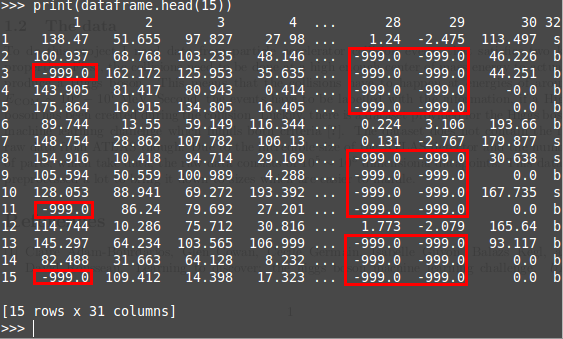
\includegraphics[width=\linewidth]{figures/datainfo_red.png}
    \caption{The first 15 datapoints from the dataset used. The red boxes mark missing data.}
    \label{fig:intro:datainfo}
\end{figure}

\subsubsection{Missing data}\label{subsubsec:intro:data:missing}

Figure \ref{fig:intro:datainfo} shows an excerpt from the dataset.
Note, that there are some points of data, which have a value of $-999.0$ in some columns, eventhough other datapoints are far off from that value.
Taking a closer look at the documentation of the data~\cite{adam2014learning} we see that some columns contain data, which is related to particle jets produced during the collision.
Events, in which no jets, or only one jet respectively, were produced, have missing data in some columns.
There were 568698 events, in which one or less jets were produced.
This results in those events having missing data in columns 5, 6, 7, 13, 27, 28 and 29.
During 320850 events there were no jets at all.
Those events have additional missing data in columns 24, 25 and 26.
To deal with this missing data, we will have to separate the events by the number of jets produced.

Unfortunately there is more missing data.
Column 1 contains data for the mass of a possible candidate for a Higgs boson.
The documentation for this columns says:\\
\\
\textit{"The estimated mass $m_H$ of the Higgs boson candidate, obtained through a probabilistic phase space integration (may be undefined if the topology of the event is too far from the expected topology)"}\\
\\
Therefore the missing data in this column is not directly related to the number of jets produced.
It is also not related to the label of the event (signal or background).
There are 122143 events with missing data in this column.
Thus this column will need to be treated separately.

    \section{The Implementation}\label{sec:code}

Next we want to take a look at how the problem was actually approached.

\subsection{Software prerequisites}\label{subsec:code:prereq}

The code has been written in python 3 and has been tested in python 3.5 on the Hyak HPC cluster at the University of Washington.
To read and manipulate the data the numpy and pandas packages are needed.
The data has been further preprocessed with functions from the sklearn package.
The neural network has been created and trained with keras using the tensorflow backend.

\subsection{Setting the options}\label{subsec:code:flags}

There are multiple ways to deal with the missing data in the dataset.
The user can choose which way should be done by setting the corresponding options when running the code via the terminal.
The usage looks like:

\texttt{python3 src/main.py <options>}

\noindent The options can be one or more of the following:

\begin{itemize}
\item \texttt{IGNORE\_MASS\_DATA}:
If this option is set, the column containing the Higgs candidate mass will be ignored completely when training the neural network. This option prevents any events from being deleted but decreases the input dimension.
\item \texttt{REMOVE\_HIGGS\_NAN}:
If this option is set, those events with missing data for the Higgs candidate mass will be deleted. This option decreases the number of total events but keeps the input dimension as it is.
\item \texttt{SIMPLE\_IMPUTE}:
This option will impute the missing data in the Higgs candidate mass with the physical value of the Higgs mass of $125.18$\;GeV \cite{tanabashi2018review}. This keeps the number of events and the input dimension unchanged, but approximates data.
\item \texttt{IGNORE\_MULTIJET\_DATA}:
If this option is set, all columns containing data, which is only defined if the number of jets is greater than one, will be ignored. Events with no jets produced will be deleted. This option reduces the number of events and the input dimension.
\item \texttt{IGNORE\_JET\_DATA}:
If this option is set, all columns containing jet data will be ignored. This keeps the number of events constant but reduces the input dimension even further than the previous option.
\end{itemize}

\subsection{Reading the data}\label{subsec:code:reading}

After the options have been set, the dataset has to be read by the program.
To do this, the \texttt{read\_csv} function from pandas is used.\footnote{In this report I will be skipping parts of the code which are not very instructive, such as error handling and garbage collection.}
\\
\\
\noindent\texttt{datafile = "data/data.csv"\\
dataframe = pd.read\_csv(datafile, header=None)}
\\
\\
Next the irrelevant data from the original challenge as well as the header of the data need to be removed.
\\
\\
\noindent\texttt{del dataframe[KAGGLE\_WEIGHT\_INDEX]\\
del dataframe[KAGGLE\_SET\_INDEX]\\
del dataframe[WEIGHT\_INDEX]\\
del dataframe[EVENTID\_INDEX]\\
dataframe = dataframe.iloc[1:]}
\\
\\
To further handle the data, we need to convert it from string to float and replace the -999.0 values by \texttt{NaN}, so it does not get confused with actually relevant data points.
The labels also have to be converted to numerical values in order to be given to the neural network.
I chose 1 to be the value for the signal label and 0 the value for the background label.
\\
\\
\noindent\texttt{dataframe = dataframe.apply(pd.to\_numeric, errors='ignore')\\
dataframe = dataframe.replace($\{$-999.0: np.NaN$\}$)\\
dataframe[LABEL\_INDEX] = 1 - pd.factorize(dataframe[LABEL\_INDEX])[0]}

\subsection{Preprocessing the data}\label{subsec:code:prepro}

Now the data is ready for actual preprocessing.
First we will take care of the missing data.
Depending on what options are set, the missing data for the jet productions are handled accordingly.
\\
\\
\noindent\texttt{if IGNORE\_JET\_DATA:\\
\indent for i in SOLOJET\_INDEX:\\
\indent\indent del dataframe[i]\\
\indent for j in MULTIJET\_INDEX:\\
\indent\indent del dataframe[j]\\
elif IGNORE\_MULTIJET\_DATA:\\
\indent for i in MULTIJET\_INDEX:\\
\indent\indent del dataframe[i]\\
\indent dataframe = dataframe[dataframe[JETNUMBER\_INDEX] > 0]\\
else:\\
\indent dataframe = dataframe[dataframe[JETNUMBER\_INDEX] > 1]}
\\
\\
Afterwards we can take care of the missing data in the Higgs candidate mass.
\\
\\
\texttt{if IGNORE\_MASS\_DATA:\\
\indent del dataframe[DER\_MASS\_INDEX]\\
elif REMOVE\_HIGGS\_NAN:\\
\indent dataframe.dropna(inplace=True)\\
elif SIMPLE\_IMPUTE:\\
\indent dataframe.fillna(PHYSICAL\_HIGGS\_MASS, inplace=True)}
\\
\\
Next we can convert the pandas dataframe into a numpy matrix and use the MinMaxScaler from the sklearn package to normalize the data.
\\
\\
\texttt{data\_matrix = dataframe.as\_matrix().astype(np.float)\\
scaler = MinMaxScaler()\\
scaler.fit(data\_matrix)\\
print("Normalizing data.")\\
data\_matrix\_norm = scaler.transform(data\_matrix)}
\\
\\
For the split between test and training data, good results could be achieved with a 85/15 split.
\\
\\
\texttt{target = data\_matrix\_norm[:, -1]\\
train = data\_matrix\_norm[:, :-1]\\
x\_train, x\_test, y\_train, y\_test = train\_test\_split(train, target,\\
\indent test\_size=0.15, random\_state=1)}
\\
\\
With that out of the way, the data is ready to be used to train the neural network.

\subsection{Training the network}\label{subsec:code:training}

The next question to ask ourselves is how to actually design the neural network.
How many input neurons should we use?
How many hidden layers should we use?
How many neurons per layer should we use?\\
After some experimenting with those parameters and doing some reading I found the best results with the following blueprint:
The number of input neurons should be equal to the dimension of the data.
Their output type should be a rectified linear unit (ReLU).
After that there should be one hidden layer, with $(\text{dim} + 1) / 2$ neurons in it.
Their output type should be a ReLU as well.
Finally there is one output neuron of the sigmoid type, since it is a binary classification problem.
The model is trained using the binary crossentropy as loss function and the \texttt{rmsprop} optimizer.
The model is trained on the \texttt{x\_train} and \texttt{y\_train} data for 20 epochs and then evaluated on the \texttt{x\_test} and \texttt{y\_test} data.\\
The implementation of this procedure with keras is rather simple and given below.
\\
\\
\texttt{model = Sequential()\\
mean = (input\_dim\_ + 1) // 2\\
model.add(Dense(input\_dim\_, input\_dim=input\_dim\_, activation='relu'))\\
model.add(Dense(mean, activation='relu'))\\
model.add(Dense(1, activation='sigmoid'))\\
model.compile(loss='binary\_crossentropy', optimizer='rmsprop',\\
\indent metrics=['accuracy'])\\
model.fit(x\_train, y\_train, epochs=20, batch\_size=128)\\
loss\_and\_metrics = model.evaluate(x\_test, y\_test, batch\_size=128)}

    \section{Results}\label{sec:results}

The resulting score on the test data depends on the design of the neural network, as well as on the way, the missing data is handled.
The first few times running the code I used a way bigger network (multiple hidden layers with 64+ neurons per layer).
Interestingly this gave worse results than the final design.
The results produced by the bigger network while ignoring all jet and Higgs candidate mass data were in the 70-75\% range.
Improving the network's design and using different ways to deal with missing data brought the accuracy of the model up significantly.
The table below shows the score on the test data as well as the value of the loss function for all different ways of dealing with missing data.

\begin{table}[H]

\centering
\begin{tabular}{|c|c|c|c|}
\hline
Jet data option					& Mass data	option			& Loss function	& Accuracy	\\
\hline
\texttt{IGNORE\_JET\_DATA}		& \texttt{IGNORE\_MASS\_DATA}	& 0.3851		& 0.8246	\\
\texttt{IGNORE\_JET\_DATA}		& \texttt{REMOVE\_HIGGS\_NAN}	& 0.4122		& 0.8107	\\
\texttt{IGNORE\ JET\_DATA}		& \texttt{SIMPLE\_IMPUTE}		& 0.3765		& 0.8303	\\
\hline
\texttt{IGNORE\_MULTIJET\_DATA}& \texttt{IGNORE\_MASS\_DATA}	& 0.4023		& 0.8149	\\
\texttt{IGNORE\_MULTIJET\_DATA}& \texttt{REMOVE\_HIGGS\_NAN}	& 0.4082		& 0.8171	\\
\texttt{IGNORE\_MULTIJET\_DATA}& \texttt{SIMPLE\_IMPUTE}		& 0.3982		& 0.8187	\\
\hline
\texttt{None}					& \texttt{IGNORE\_MASS\_DATA}	& 0.3758		& 0.8357	\\
\texttt{None}					& \texttt{REMOVE\_HIGGS\_NAN}	& 0.3648		& 0.8393	\\
\texttt{None}					& \texttt{SIMPLE\_IMPUTE}		& 0.3500		& 0.8501	\\
\hline
\end{tabular}
\caption{Results of the final model.}
\end{table}

These results show us, that the model can give more accurate predictions, if we use higher dimensional data, eventhough we lose a lot of events that way.
Using only the data of those events, in which two or more jets have been produced, together with the physical Higgs mass imputed for the missing data in that column brings the accuracy up to about 85\%, which is a significant impovement from the beginning 70-75\%.

    \section{Closing remarks and outlook}\label{sec:outlook}

We have seen that even a simple model, which has been trained without any knowledge about high energy particle physics or relativistic kinematics, can perform quite well in classifying collision events.
We have also seen that only a few steps of optimization can bring up the performance of the neural network significantly.
Eventhough we get some nice results, the model is far from perfect and does not compare to the ones actually used for the challenge or research done at CERN.
But even within the scope of this project there are still some ways to improve on the project.
One idea, which I did not manage to implement yet is to improve the imputer for the missing Higgs candidate mass data by training a separate regression model on the events with valid data to predict a value for the missing data.
Another way to improve is to implement some of the statistical tweaks mentioned by Balázs Kégl in his talk, in which he introduces the challenge.\footnote{http://opendata.cern.ch/record/330}


    
    \clearpage
    
    \bibliography{ref}

\end{document}